
%%%%%%%%%%%%%%%%%%%%%%%%%%%%%%%%%%%%%%%%
%             Background               %
%%%%%%%%%%%%%%%%%%%%%%%%%%%%%%%%%%%%%%%%

\begin{frame}
  \frametitle{\kd trees}
  \framesubtitle{Introduction}

  \begin{itemize}
    \item Partition $k$-dimensional space
    \item Recursively splits point clouds with hyperplanes at each node
      \begin{itemize}
        \item Hyperplanes usually orthogonal to coordinate axis
      \end{itemize}
    \item Binary search trees are the one-dimensional versions of \kd trees
  \end{itemize}
\end{frame}

\begin{frame}
  \frametitle{\kd trees}
  \framesubtitle{Example: $k=1$}

  \begin{figure}
    \centering
    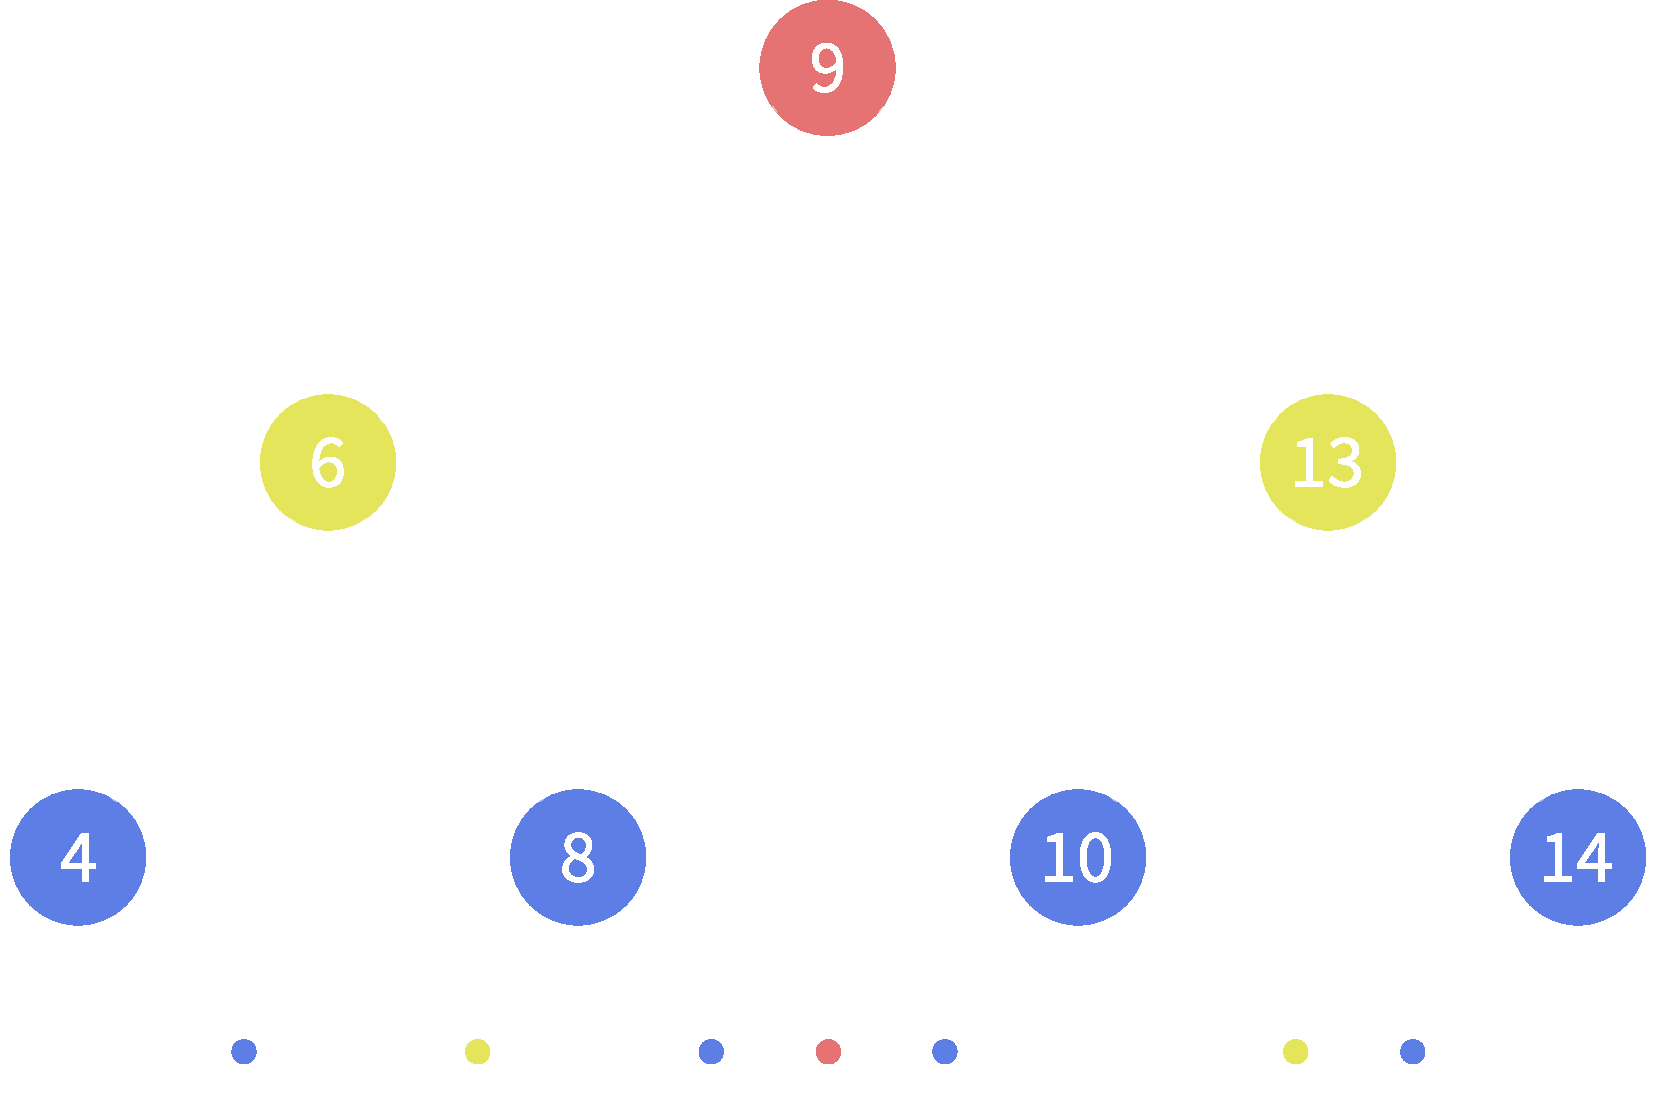
\includegraphics[width=0.7\textwidth]{BST.pdf}
  \end{figure}
  
\end{frame}

\begin{frame}
  \frametitle{\kd trees}
  \framesubtitle{Example: $k=2$}
  
  \begin{figure}
    \centering
    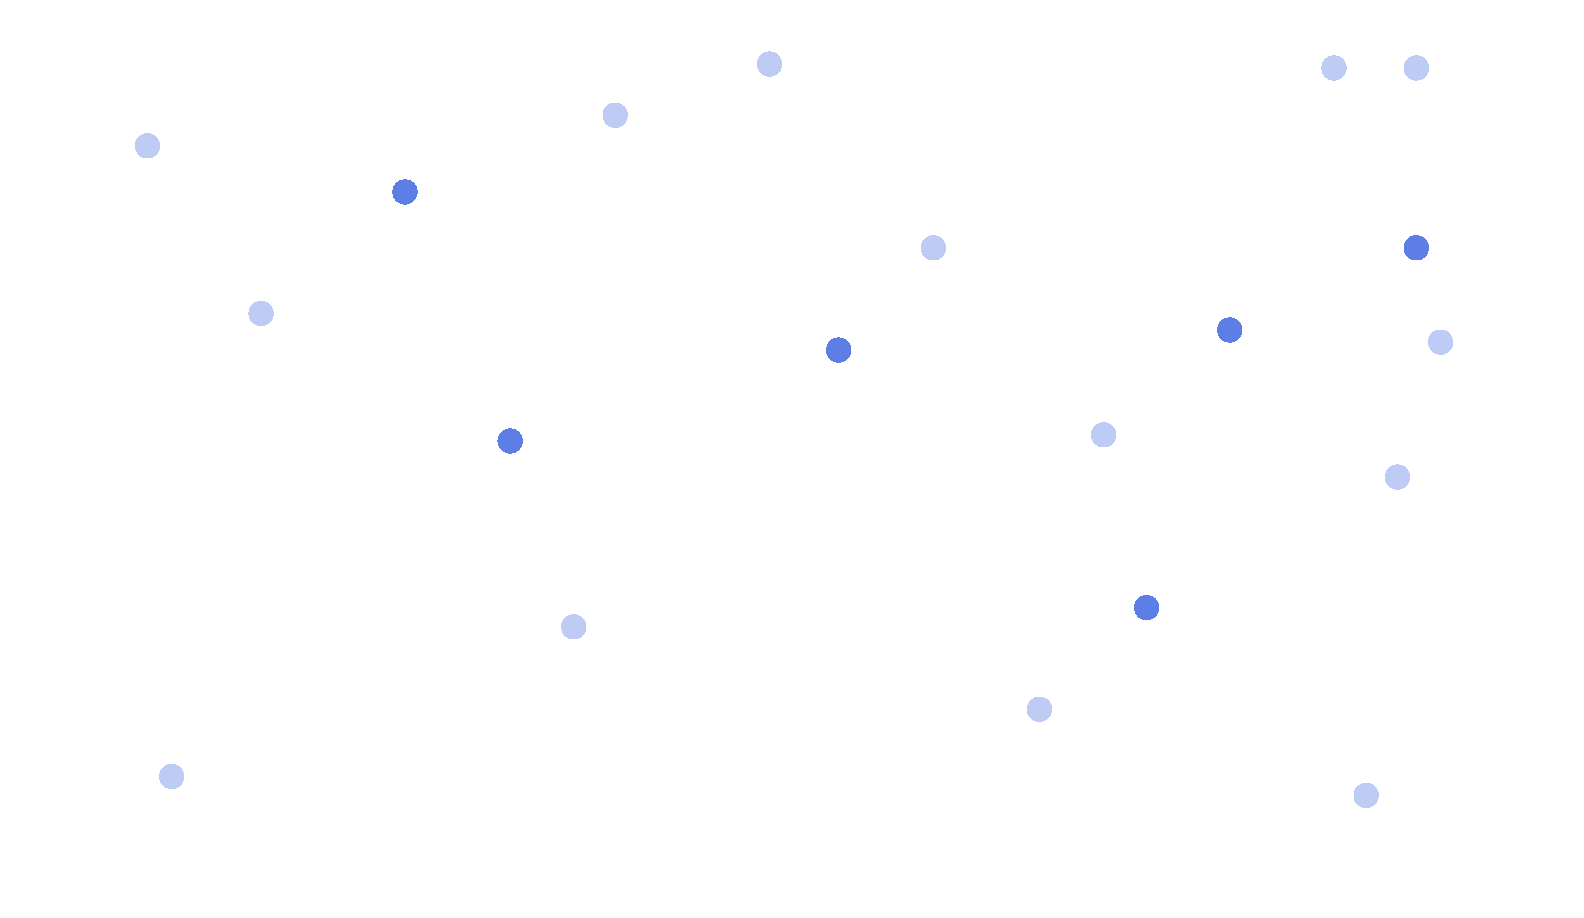
\includegraphics[width=0.73\textwidth]{2dkdtree.pdf}
  \end{figure}

\end{frame}

\begin{frame}
  \frametitle{\kd trees}
  \framesubtitle{Example: $k=3$}
  
  \begin{figure}
    \centering
    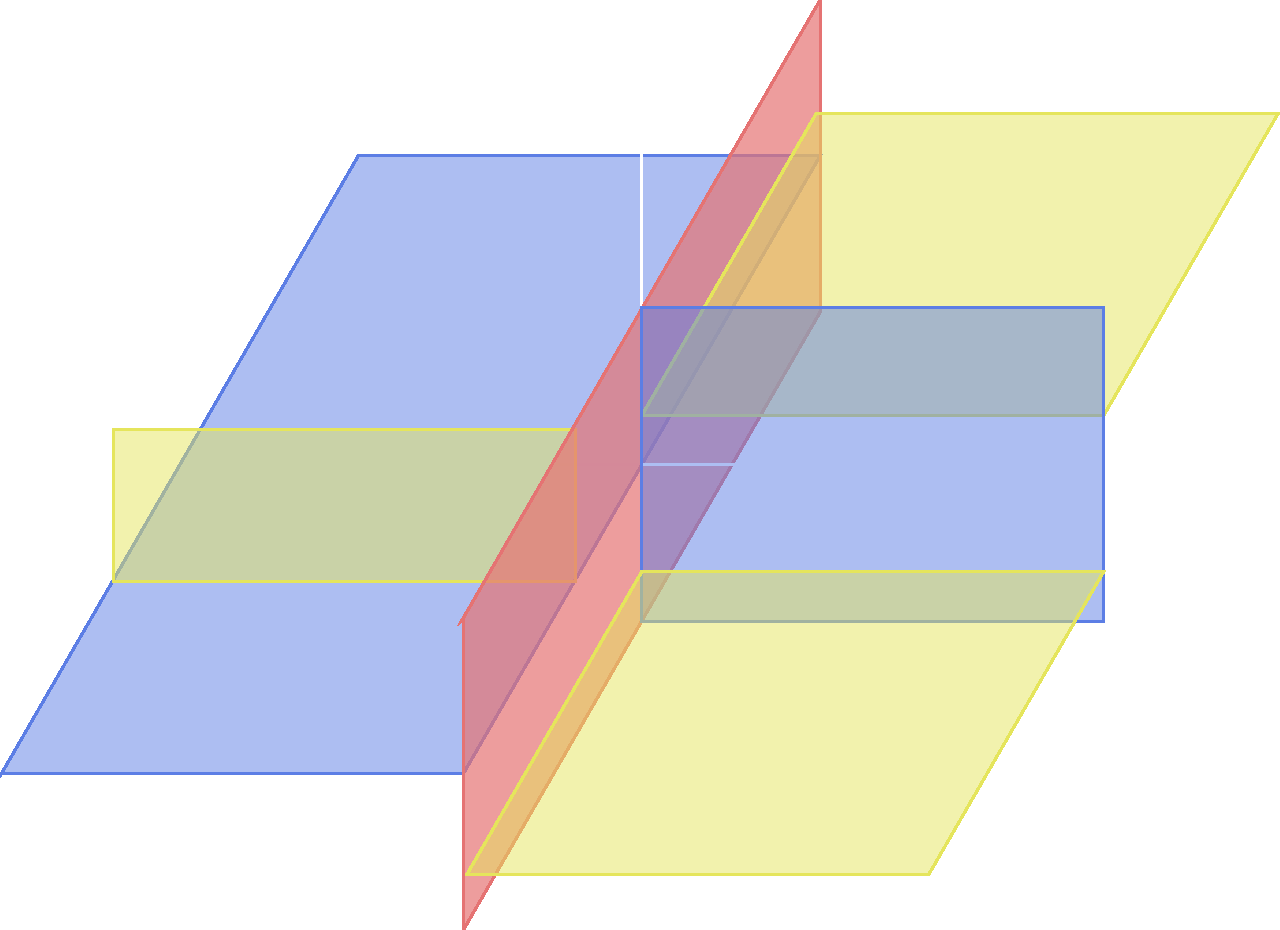
\includegraphics[width=0.6\textwidth]{3dkdtree.pdf}
  \end{figure}

\end{frame}

\begin{frame}
  \frametitle{\kd trees}
  \framesubtitle{Nearest neighbor search}

  \begin{enumerate}
    \item Given a point, $p$, rescursively move down the tree by computing the points orientation relative to the 
      hyperplane $t$ given by $p - \text{proj}_t(p)$
    \item At each node, compare the distance of the query point to the node's splitting point with the distance
      of the current nearest neighbor, if smaller, update nearest neighbor candidate
    \item Upon completion of recursive call, compare the distance of current nearest neighbor 
      candidate to the point with the distance to the hyperplane $\|p - \text{proj}_t(p)\|$; 
      if it is larger, search the other child branch of the node
  \end{enumerate}

\end{frame}

\begin{frame}
  \frametitle{\kd trees}
  \framesubtitle{Nanoflann}

  \begin{itemize}
    \item Header-only C++ \kd tree implementation that supports k-nearest neighbor and radius search with 
      L1 or L2 metric
    \item Utilizes curiously recurring template pattern and inlined functions for high performance
    \item Used for nearest neighbor search in our ZENO/Walk-on-Spheres implementation 
  \end{itemize}

\end{frame}

%%%%%%%%%%%%%%%%%%%%%%%%%%%%%%%%%%%%%%%%
%             Limitations              %
%%%%%%%%%%%%%%%%%%%%%%%%%%%%%%%%%%%%%%%%

\begin{frame}
  \frametitle{\kd trees}
  \framesubtitle{Limitations of trees}

  \begin{itemize}
    \item Memory access pattern when searching tree is unpredictable
      \begin{itemize}
        \item Can't align contiguous blocks with temporal locality
        \item Difficult to prefetch memory
      \end{itemize}
    \item Does not maintain spatially locallity within memory
  \end{itemize}
\end{frame}

\begin{frame}
  \frametitle{\kd trees}
  \framesubtitle{Height and its GPU limitations}

  \begin{columns}[T]
    \begin{column}{.5\textwidth}
      \begin{block}{}%
        {\color{white} \bullet\hspace{1mm} Costly edge cases lead to large variance in search dereferences 
          and time\\\vspace{0.5cm}
        
        \bullet\hspace{1mm} Queries require at least $O(\lg n)$ pointer dereferences\\\vspace{0.5cm}

      \bullet\hspace{1mm} Only single subpsace look ahead during search}
      \end{block}
    \end{column}
    \begin{column}{.5\textwidth}
      \begin{block}{}
        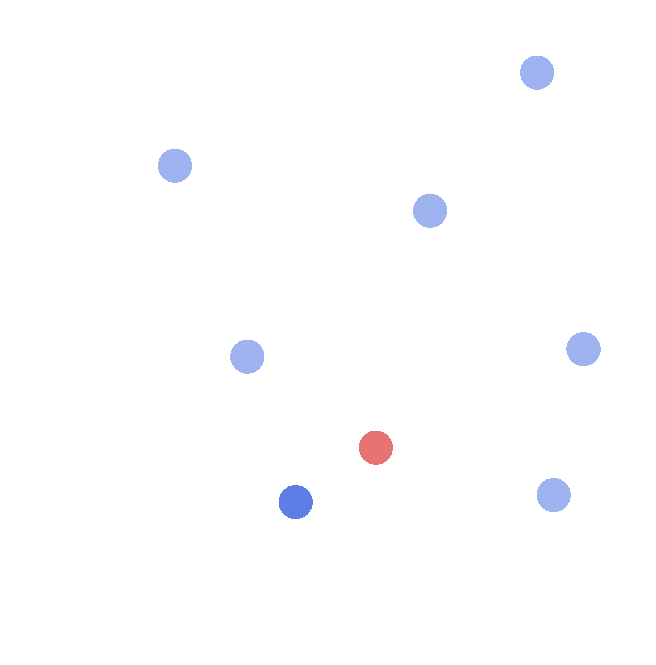
\includegraphics[width=0.85\textwidth]{nn_adjaceny_simple.pdf}
      \end{block}
    \end{column}
  \end{columns}
\end{frame}
